% answers.tex —— 2019 年·天津卷·文科 · 参考答案与详细解析片段
% 由 tools/generate_projects.py 依来源总账自 2019/2019_数学真题_天津卷文_试题.md + 2019/2019_数学真题_天津卷文_解析正文.md + 2019/2019_数学真题_天津卷文_答案要点.md 生成，勿手改（改源 MD 后重跑）

\begin{gktip}
固定源没有答案页；以下为非官方推导，不能称为官方答案。
\end{gktip}

\gkpart{一、选择题}

\begin{answer}
\gksolhead{1}{}

\textbf{题目}：

设集合 $A = \{-1, 1, 2, 3, 5\}$, $B = \{2, 3, 4\}$, $C = \{x \in \mathbb{R} \mid 1 \leqslant x < 3\}$, 则 $(A \cap C) \cup B =$（ ）。

(A) $\{2\}$　(B) $\{2, 3\}$　(C) $\{-1, 2, 3\}$　(D) $\{1, 2, 3, 4\}$

\Needspace{4\baselineskip}
\textbf{解析}

由集合交集与并集的定义：
已知 $A = \{-1, 1, 2, 3, 5\}$, $C = \{x \in \mathbb{R} \mid 1 \leqslant x < 3\}$,
则 $A \cap C = \{1, 2\}$.
\Needspace{5\baselineskip}
进而由集合 $B = \{2, 3, 4\}$, 计算并集得：
\nopagebreak[4]
\[(A \cap C) \cup B = \{1, 2\} \cup \{2, 3, 4\} = \{1, 2, 3, 4\}.\]
故选 \textbf{D}。

\gkanswer{答案：D}

\end{answer}
\begin{answer}
\gksolhead{2}{}

\textbf{题目}：

\Needspace{5\baselineskip}
设变量 $x, y$ 满足约束条件
\nopagebreak[4]
\[
\begin{cases}
x + y - 2 \leqslant 0, \\
x - y + 2 \geqslant 0, \\
x \geqslant -1, \\
y \geqslant -1,
\end{cases}
\]
则目标函数 $z = -4x + y$ 的最大值为（ ）。

(A) $2$　(B) $3$　(C) $5$　(D) $6$

\Needspace{4\baselineskip}
\textbf{解析}

绘制不等式组表示的平面可行域：
\Needspace{5\baselineskip}
不等式组为
\nopagebreak[4]
\[
\begin{cases}
x + y - 2 \leqslant 0, \\
x - y + 2 \geqslant 0, \\
x \geqslant -1, \\
y \geqslant -1.
\end{cases}
\]
其边界直线交点构成四边形凸多边形区域，各顶点坐标分别为：
\begin{itemize}
\item 直线 $x = -1$ 与 $y = -1$ 的交点为 $(-1, -1)$；
\item 直线 $x = -1$ 与 $x - y + 2 = 0$ 的交点为 $(-1, 1)$；
\item 直线 $x + y - 2 = 0$ 与 $x - y + 2 = 0$ 的交点为 $(0, 2)$；
\item 直线 $x + y - 2 = 0$ 与 $y = -1$ 的交点为 $(3, -1)$。
\end{itemize}
将各顶点代入目标函数 $z = -4x + y$：
\begin{itemize}
\item 代入 $(-1, -1)$ 得 $z = -4(-1) + (-1) = 3$；
\item 代入 $(-1, 1)$ 得 $z = -4(-1) + 1 = 5$；
\item 代入 $(0, 2)$ 得 $z = -4(0) + 2 = 2$；
\item 代入 $(3, -1)$ 得 $z = -4(3) + (-1) = -13$。
\end{itemize}
比较可知，$z$ 的最大值为 $5$，在点 $(-1, 1)$ 处取得。
故选 \textbf{C}。

\gkanswer{答案：C}

\end{answer}
\begin{answer}
\gksolhead{3}{}

\textbf{题目}：

设 $x \in \mathbb{R}$, 则“$0 < x < 5$”是“$|x - 1| < 1$”的（ ）。

(A) 充分而不必要条件　(B) 必要而不充分条件  
(C) 充要条件　(D) 既不充分也不必要条件

\Needspace{4\baselineskip}
\textbf{解析}

\Needspace{5\baselineskip}
解绝对值不等式：
\nopagebreak[4]
\[|x - 1| < 1 \iff -1 < x - 1 < 1 \iff 0 < x < 2.\]
因为 $(0, 2) \subsetneq (0, 5)$，所以由 $|x - 1| < 1$ 可以推出 $0 < x < 5$；
但由 $0 < x < 5$ 不能推出 $|x - 1| < 1$（例如取 $x = 3$ 时满足 $0 < x < 5$，但 $|3 - 1| = 2 \not< 1$）。
因此，“$0 < x < 5$”是“$|x - 1| < 1$”的必要而不充分条件。
故选 \textbf{B}。

\gkanswer{答案：B}

\end{answer}
\begin{answer}
\gksolhead{4}{}

\textbf{题目}：

阅读如图的程序框图, 运行相应的程序, 输出 $S$ 的值为（ ）。
\nopagebreak[4]
\begin{center}\begin{tikzpicture}[>=latex, font=\small, scale=0.9]
  \tikzstyle{startstop} = [draw, rounded corners=6pt, minimum width=1.6cm, minimum height=0.6cm, text centered]
  \tikzstyle{io} = [draw, trapezium, trapezium left angle=70, trapezium right angle=110, minimum width=1.8cm, minimum height=0.6cm, text centered]
  \tikzstyle{process} = [draw, minimum width=2.0cm, minimum height=0.6cm, text centered]
  \tikzstyle{decision} = [draw, diamond, aspect=2.2, minimum width=2.4cm, minimum height=0.7cm, text centered]
  \tikzstyle{arrow} = [thick, ->]

  \node (start) [startstop] at (0, 0) {开始};
  \node (init) [process] at (0, -0.95) {$i = 1,\ S = 0$};
  \node (dec1) [decision] at (0, -2.15) {$i$ 为偶数?};
  \node (proc1) [process] at (0, -3.35) {$j = \dfrac{i}{2}$};
  \node (proc2) [process] at (0, -4.35) {$S = S + i \cdot 2^j$};
  \node (odd) [process] at (2.2, -3.35) {$S = S + i$};
  \node (inc) [process] at (0, -5.35) {$i = i + 1$};
  \node (dec2) [decision] at (0, -6.45) {$i \geqslant 4$?};
  \node (out) [io] at (0, -7.6) {输出 $S$};
  \node (stop) [startstop] at (0, -8.45) {结束};

  \draw[arrow] (start) -- (init);
  \draw[arrow] (init) -- (dec1);
  \draw[arrow] (dec1) -- node[right] {是} (proc1);
  \draw[arrow] (proc1) -- (proc2);
  \draw[arrow] (proc2) -- (inc);
  \draw[arrow] (dec1.east) -| node[above, pos=0.3] {否} (odd.north);
  \draw[arrow] (odd.south) |- ([yshift=0.25cm]inc.north);
  \draw[arrow] (inc) -- (dec2);
  \draw[arrow] (dec2) -- node[right] {是} (out);
  \draw[arrow] (out) -- (stop);

  \draw[arrow] (dec2.west) -- node[above] {否} ++(-1.6, 0) |- ([yshift=0.2cm]dec1.north);
\end{tikzpicture}
\end{center}
\nopagebreak[4]
(A) $5$　(B) $8$　(C) $24$　(D) $29$

\Needspace{4\baselineskip}
\textbf{解析}

按照程序框图逐步追踪变量的变化过程：
\begin{itemize}
\item 初始时，$i = 1, S = 0$；
\item 判断 $i$ 为偶数：$1$ 为奇数，走“否”分支，计算
\end{itemize}
\nopagebreak[4]
\[S = S + i = 0 + 1 = 1,\]
  执行 $i = i + 1 = 2$；
  判断 $i \geqslant 4$：$2 \geqslant 4$ 不成立，走“否”分支循环；
\begin{itemize}
\item 判断 $i$ 为偶数：$2$ 为偶数，走“是”分支，计算
\end{itemize}
\nopagebreak[4]
\[j = \frac{i}{2} = 1,\quad S = S + i \cdot 2^j = 1 + 2 \cdot 2^1 = 5,\]
  执行 $i = i + 1 = 3$；
  判断 $i \geqslant 4$：$3 \geqslant 4$ 不成立，走“否”分支循环；
\begin{itemize}
\item 判断 $i$ 为偶数：$3$ 为奇数，走“否”分支，计算
\end{itemize}
\nopagebreak[4]
\[S = S + i = 5 + 3 = 8,\]
  执行 $i = i + 1 = 4$；
  判断 $i \geqslant 4$：$4 \geqslant 4$ 成立，走“是”分支退出循环；
\begin{itemize}
\item 输出 $S = 8$.
\end{itemize}
故选 \textbf{B}。

\gkanswer{答案：B}

\end{answer}
\begin{answer}
\gksolhead{5}{}

\textbf{题目}：

已知 $a = \log_2 7$, $b = \log_3 8$, $c = 0.3^{0.2}$, 则 $a, b, c$ 的大小关系为（ ）。

(A) $c < b < a$　(B) $a < b < c$　(C) $b < c < a$　(D) $c < a < b$

\Needspace{4\baselineskip}
\textbf{解析}

分别估算 $a, b, c$ 的数值范围：
\begin{itemize}
\item 对于 $a = \log_2 7$：因为 $4 < 7 < 8$，且对数函数 $y = \log_2 x$ 单调递增，所以
\end{itemize}
\nopagebreak[4]
\[2 = \log_2 4 < a < \log_2 8 = 3;\]
\begin{itemize}
\item 对于 $b = \log_3 8$：因为 $3 < 8 < 9$，且对数函数 $y = \log_3 x$ 单调递增，所以
\end{itemize}
\nopagebreak[4]
\[1 = \log_3 3 < b < \log_3 9 = 2;\]
\begin{itemize}
\item 对于 $c = 0.3^{0.2}$：底数 $0.3 \in (0, 1)$，指数函数 $y = 0.3^x$ 在 $\mathbb{R}$ 上单调递减。
\end{itemize}
\Needspace{5\baselineskip}
  因为 $0 < 0.2 < 1$，所以
\nopagebreak[4]
\[0.3 = 0.3^1 < c < 0.3^0 = 1.\]
综合上述估算，可知 $c \in (0.3, 1)$，$b \in (1, 2)$，$a \in (2, 3)$，因此 $c < b < a$。
故选 \textbf{A}。

\gkanswer{答案：A}

\end{answer}
\begin{answer}
\gksolhead{6}{}

\textbf{题目}：

已知抛物线 $y^2 = 4x$ 的焦点为 $F$, 准线为 $l$. 若 $l$ 与双曲线 $\dfrac{x^2}{a^2} - \dfrac{y^2}{b^2} = 1$ ($a > 0, b > 0$) 的两条渐近线分别交于点 $A$ 和点 $B$, 且 $|AB| = 4|OF|$ ($O$ 为原点), 则双曲线的离心率为（ ）。

(A) $\sqrt{2}$　(B) $\sqrt{3}$　(C) $2$　(D) $\sqrt{5}$

\Needspace{4\baselineskip}
\textbf{解析}

抛物线 $y^2 = 4x$ 的焦准距参数 $p = 2$，焦点为 $F(1, 0)$，原点到焦点的距离 $|OF| = 1$，准线 $l$ 的方程为 $x = -1$。
双曲线 $\dfrac{x^2}{a^2} - \dfrac{y^2}{b^2} = 1$ 的两条渐近线方程为 $y = \pm \dfrac{b}{a} x$。
准线 $l: x = -1$ 与两条渐近线分别交于点 $A\left(-1, \dfrac{b}{a}\right)$ 和 $B\left(-1, -\dfrac{b}{a}\right)$。
\Needspace{5\baselineskip}
线段 $AB$ 的长度为：
\nopagebreak[4]
\[|AB| = \left|\frac{b}{a} - \left(-\frac{b}{a}\right)\right| = \frac{2b}{a}.\]
\Needspace{5\baselineskip}
已知 $|AB| = 4|OF| = 4$，代入得：
\nopagebreak[4]
\[\frac{2b}{a} = 4 \implies \frac{b}{a} = 2.\]
\Needspace{5\baselineskip}
由双曲线离心率公式：
\nopagebreak[4]
\[e = \sqrt{1 + \left(\frac{b}{a}\right)^2} = \sqrt{1 + 2^2} = \sqrt{5}.\]
故选 \textbf{D}。

\gkanswer{答案：D}

\end{answer}
\begin{answer}
\gksolhead{7}{}

\textbf{题目}：

已知函数 $f(x) = A \sin(\omega x + \varphi)$ ($A > 0, \omega > 0, |\varphi| < \pi$) 是奇函数, 且 $f(x)$ 的最小正周期为 $\pi$, 将 $y = f(x)$ 的图象上所有点的横坐标伸长到原来的 $2$ 倍 (纵坐标不变), 所得图象对应的函数为 $g(x)$. 若 $g\left(\dfrac{\pi}{4}\right) = \sqrt{2}$, 则 $f\left(\dfrac{3\pi}{8}\right) =$（ ）。

(A) $-2$　(B) $-\sqrt{2}$　(C) $\sqrt{2}$　(D) $2$

\Needspace{4\baselineskip}
\textbf{解析}

已知函数 $f(x) = A \sin(\omega x + \varphi)$ ($A > 0, \omega > 0, |\varphi| < \pi$) 是奇函数，且最小正周期为 $\pi$。
由奇函数条件可知 $\varphi = 0$。
\Needspace{5\baselineskip}
由周期公式：
\nopagebreak[4]
\[\frac{2\pi}{\omega} = \pi \implies \omega = 2.\]
所以 $f(x) = A \sin(2x)$。
\Needspace{5\baselineskip}
将 $y = f(x)$ 的图象上所有点的横坐标伸长到原来的 $2$ 倍（纵坐标不变），所得图象对应的函数为
\nopagebreak[4]
\[g(x) = f\left(\frac{x}{2}\right) = A \sin\left(2 \cdot \frac{x}{2}\right) = A \sin x.\]
\Needspace{5\baselineskip}
已知 $g\left(\dfrac{\pi}{4}\right) = \sqrt{2}$，即
\nopagebreak[4]
\[A \sin\frac{\pi}{4} = A \cdot \frac{\sqrt{2}}{2} = \sqrt{2} \implies A = 2.\]
从而 $f(x) = 2 \sin(2x)$。
\Needspace{5\baselineskip}
计算 $f\left(\dfrac{3\pi}{8}\right)$ 的值：
\nopagebreak[4]
\[f\left(\frac{3\pi}{8}\right) = 2 \sin\left(2 \cdot \frac{3\pi}{8}\right) = 2 \sin\frac{3\pi}{4} = 2 \cdot \frac{\sqrt{2}}{2} = \sqrt{2}.\]
故选 \textbf{C}。

\gkanswer{答案：C}

\end{answer}
\begin{answer}
\gksolhead{8}{}

\textbf{题目}：

已知函数 $f(x) = \begin{cases} 2\sqrt{x}, & 0 \leqslant x \leqslant 1, \\ \dfrac{1}{x}, & x > 1, \end{cases}$ 若关于 $x$ 的方程 $f(x) = -\dfrac{1}{4}x + a$ ($a \in \mathbb{R}$) 恰有两个互异的实数解, 则 $a$ 的取值范围为（ ）。

(A) $\left[\dfrac{5}{4}, \dfrac{9}{4}\right]$　(B) $\left(\dfrac{5}{4}, \dfrac{9}{4}\right]$　(C) $\left(\dfrac{5}{4}, \dfrac{9}{4}\right] \cup \{1\}$　(D) $\left[\dfrac{5}{4}, \dfrac{9}{4}\right] \cup \{1\}$

\Needspace{4\baselineskip}
\textbf{解析}

方程 $f(x) = -\dfrac{1}{4}x + a$ 恰有两个互异实数解，等价于函数 $y = f(x)$ 的图象与直线 $y = -\dfrac{1}{4}x + a$ 恰有两个不同的交点。
分段考察函数 $y = f(x)$ 的图象：
(1) 当 $0 \leqslant x \leqslant 1$ 时，$f(x) = 2\sqrt{x}$，其图象是由 $(0, 0)$ 到 $(1, 2)$ 连续递增的凸弧段。
直线方程为 $y = -\dfrac{1}{4}x + a$，斜率为 $-\dfrac{1}{4} < 0$。
设差函数 $h(x) = 2\sqrt{x} - \left(-\dfrac{1}{4}x + a\right) = 2\sqrt{x} + \dfrac{1}{4}x - a$。
因为 $h(x)$ 在 $[0, 1]$ 上严格单调递增，所以直线与该弧段至多有 1 个交点。
\Needspace{5\baselineskip}
交点存在的充要条件是端点函数值异号或为零：
\nopagebreak[4]
\[h(0) \leqslant 0 \iff -a \leqslant 0 \iff a \geqslant 0,\]
\nopagebreak[4]
\[h(1) \geqslant 0 \iff 2 + \frac{1}{4} - a \geqslant 0 \iff a \leqslant \frac{9}{4}.\]
因此，当 $0 \leqslant a \leqslant \dfrac{9}{4}$ 时，直线与第一段图象恰有 1 个交点；当 $a < 0$ 或 $a > \dfrac{9}{4}$ 时，与第一段无交点。

(2) 当 $x > 1$ 时，$f(x) = \dfrac{1}{x}$。
\Needspace{5\baselineskip}
联立直线与双曲线分支：
\nopagebreak[4]
\[\frac{1}{x} = -\frac{1}{4}x + a \iff x^2 - 4ax + 4 = 0.\]
判别式为 $\Delta = (-4a)^2 - 4 \times 1 \times 4 = 16(a^2 - 1)$。
\begin{itemize}
\item 若 $\Delta = 0 \iff a = 1$（因为要求根在 $(1, +\infty)$，负根舍去），此时方程有重根 $x = 2a = 2 > 1$。
\end{itemize}
  此时在第二段恰有 1 个切点交点 $x = 2$；
  同时在第一段上，$a = 1 \in \left[0, \dfrac{9}{4}\right]$，恰有 1 个交点。
  两交点显然互异（一个在 $[0, 1]$ 内，一个为 $x = 2$），因此 $a = 1$ 满足题意。
\begin{itemize}
\item 若 $\Delta > 0 \iff a > 1$，方程有两个实数根 $x_{1,2} = 2a \pm 2\sqrt{a^2 - 1}$，满足 $x_1 x_2 = 4$。
\end{itemize}
  设二次函数 $g(x) = x^2 - 4ax + 4$：
\begin{itemize}
\item 当 $1 < a < \dfrac{5}{4}$ 时，$g(1) = 5 - 4a > 0$ 且对称轴 $2a > 2 > 1$，两根均落在 $(1, +\infty)$ 内，第二段有 2 个交点；此时 $a \in \left(1, \dfrac{5}{4}\right) \subset \left[0, \dfrac{9}{4}\right]$，第一段还有 1 个交点，总计有 3 个交点，不合题意；
\item 当 $a \geqslant \dfrac{5}{4}$ 时，$g(1) = 5 - 4a \leqslant 0$。较小根满足 $x_1 \leqslant 1$，较大根满足 $x_2 \geqslant 4 > 1$。
\end{itemize}
    因为第二段的定义域为 $x > 1$，较小根不落在第二段内，所以第二段恰有 1 个交点（即较大根 $x_2$）。
    此时要保证总交点数恰为 2，只需第一段也恰有 1 个交点，即 $a \leqslant \dfrac{9}{4}$。
    因此 $a \in \left[\dfrac{5}{4}, \dfrac{9}{4}\right]$ 均满足题意。

综合以上分析，$a$ 的取值范围为 $\left[\dfrac{5}{4}, \dfrac{9}{4}\right] \cup \{1\}$。
故选 \textbf{D}。

\gkanswer{答案：D}

\par\medskip

\end{answer}
\gkpart{二、填空题}

\begin{answer}
\gksolhead{9}{}

\textbf{题目}：

$\mathrm{i}$ 是虚数单位, 则 $\dfrac{5 - \mathrm{i}}{1 + \mathrm{i}}$ 的值为 $\underline{\phantom{XXXX}}$.

\Needspace{4\baselineskip}
\textbf{解析}

\Needspace{5\baselineskip}
利用复数的除法法则，将分母实数化：
\nopagebreak[4]
\[\frac{5 - \mathrm{i}}{1 + \mathrm{i}} = \frac{(5 - \mathrm{i})(1 - \mathrm{i})}{(1 + \mathrm{i})(1 - \mathrm{i})} = \frac{5 - 5\mathrm{i} - \mathrm{i} + \mathrm{i}^2}{1 - \mathrm{i}^2} = \frac{5 - 6\mathrm{i} - 1}{1 - (-1)} = \frac{4 - 6\mathrm{i}}{2} = 2 - 3\mathrm{i}.\]

\gkanswer{答案：$2 - 3\mathrm{i}$}

\end{answer}
\begin{answer}
\gksolhead{10}{}

\textbf{题目}：

设 $x \in \mathbb{R}$, 使不等式 $3x^2 + x - 2 < 0$ 成立的 $x$ 的取值范围为 $\underline{\phantom{XXXX}}$.

\Needspace{4\baselineskip}
\textbf{解析}

解一元二次不等式 $3x^2 + x - 2 < 0$：
\Needspace{5\baselineskip}
对二次三项式因式分解：
\nopagebreak[4]
\[(3x - 2)(x + 1) < 0.\]
二次项系数 $3 > 0$，抛物线开口向上，小于零的解集在两根之间。
方程 $(3x - 2)(x + 1) = 0$ 的两根分别为 $x = -1$ 和 $x = \dfrac{2}{3}$。
因此不等式的解集为 $\left(-1, \dfrac{2}{3}\right)$。

\gkanswer{答案：$\left(-1, \dfrac{2}{3}\right)$}

\end{answer}
\begin{answer}
\gksolhead{11}{}

\textbf{题目}：

曲线 $y = \cos x - \dfrac{x}{2}$ 在点 $(0, 1)$ 处的切线方程为 $\underline{\phantom{XXXX}}$.

\Needspace{4\baselineskip}
\textbf{解析}

已知函数 $y = \cos x - \dfrac{x}{2}$。
\Needspace{5\baselineskip}
对其求导得：
\nopagebreak[4]
\[y' = -\sin x - \frac{1}{2}.\]
\Needspace{5\baselineskip}
将切点的横坐标 $x = 0$ 代入导函数，得到切线的斜率：
\nopagebreak[4]
\[k = y'(0) = -\sin 0 - \frac{1}{2} = -\frac{1}{2}.\]
\Needspace{5\baselineskip}
又切线经过点 $(0, 1)$，根据点斜式方程：
\nopagebreak[4]
\[y - 1 = -\frac{1}{2}(x - 0) \iff y = -\frac{1}{2}x + 1 \iff x + 2y - 2 = 0.\]

\gkanswer{答案：$x + 2y - 2 = 0$}

\end{answer}
\begin{answer}
\gksolhead{12}{}

\textbf{题目}：

已知四棱锥的底面是边长为 $\sqrt{2}$ 的正方形, 侧棱长均为 $\sqrt{5}$. 若圆柱的一个底面的圆周经过四棱锥四条侧棱的中点, 另一个底面的圆心为四棱锥底面的中心, 则该圆柱的体积为 $\underline{\phantom{XXXX}}$.

\Needspace{4\baselineskip}
\textbf{解析}

设四棱锥为 $P-ABCD$，底面正方形 $ABCD$ 的边长为 $\sqrt{2}$，侧棱长为 $\sqrt{5}$。
底面中心记为 $O$，连接 $AC$ 与 $BD$ 交于 $O$。
由正方形性质，对角线长 $AC = \sqrt{(\sqrt{2})^2 + (\sqrt{2})^2} = 2$，
因此底面中心到各顶点的距离为 $OA = \frac{1}{2} AC = 1$。
四棱锥为正四棱锥，高线 $PO \perp \text{\text{平面} } ABCD$。
\Needspace{5\baselineskip}
在直角三角形 $\triangle POA$ 中，由勾股定理得高线长：
\nopagebreak[4]
\[PO = \sqrt{PA^2 - OA^2} = \sqrt{(\sqrt{5})^2 - 1^2} = \sqrt{4} = 2.\]
由题意，圆柱的一个底面的圆心为底面中心 $O$，另一个底面的圆周经过四棱锥四条侧棱的中点。
设四条侧棱的中点构成的截面与高线 $PO$ 交于 $O'$，则 $O'$ 为 $PO$ 的中点，且 $PO' \perp \text{\text{平面} } ABCD$。
\Needspace{5\baselineskip}
各侧棱中点到高线 $PO$ 的距离均为底面对角线半长的一半，即
\nopagebreak[4]
\[r = \frac{1}{2} OA = \frac{1}{2} \times 1 = \frac{1}{2}.\]
因此圆柱的底面半径为 $r = \dfrac{1}{2}$。
\Needspace{5\baselineskip}
圆柱的高等于线段 $OO'$ 的长度，即
\nopagebreak[4]
\[h = OO' = \frac{1}{2} PO = \frac{1}{2} \times 2 = 1.\]
\Needspace{5\baselineskip}
根据圆柱的体积公式：
\nopagebreak[4]
\[V = \pi r^2 h = \pi \left(\frac{1}{2}\right)^2 \times 1 = \frac{\pi}{4}.\]

\gkanswer{答案：$\dfrac{\pi}{4}$}

\end{answer}
\begin{answer}
\gksolhead{13}{}

\textbf{题目}：

设 $x > 0, y > 0, x + 2y = 5$, 则 $\dfrac{(x + 1)(2y + 1)}{\sqrt{xy}}$ 的最小值为 $\underline{\phantom{XXXX}}$.

\Needspace{4\baselineskip}
\textbf{解析}

\Needspace{5\baselineskip}
展开分式的分子部分：
\nopagebreak[4]
\[(x + 1)(2y + 1) = 2xy + x + 2y + 1.\]
\Needspace{5\baselineskip}
已知 $x + 2y = 5$，代入分子可得：
\nopagebreak[4]
\[(x + 1)(2y + 1) = 2xy + 5 + 1 = 2xy + 6.\]
\Needspace{5\baselineskip}
因此待求最值的表达式可以写为：
\nopagebreak[4]
\[\frac{(x + 1)(2y + 1)}{\sqrt{xy}} = \frac{2xy + 6}{\sqrt{xy}} = 2\sqrt{xy} + \frac{6}{\sqrt{xy}}.\]
\Needspace{5\baselineskip}
因为 $x > 0, y > 0$，根据基本不等式：
\nopagebreak[4]
\[5 = x + 2y \geqslant 2\sqrt{x \cdot 2y} = 2\sqrt{2xy},\]
\Needspace{5\baselineskip}
两边除以 $2\sqrt{2}$ 并平方得：
\nopagebreak[4]
\[\sqrt{2xy} \leqslant \frac{5}{2} \implies 2xy \leqslant \frac{25}{4} \implies xy \leqslant \frac{25}{8}.\]
设 $t = \sqrt{xy}$，则 $0 < t \leqslant \dfrac{5\sqrt{2}}{4}$。
构造对勾函数 $g(t) = 2t + \dfrac{6}{t}$ ($t > 0$)。
由均值不等式，$g(t) \geqslant 2\sqrt{2t \cdot \frac{6}{t}} = 2\sqrt{12} = 4\sqrt{3}$，
等号成立当且仅当 $2t = \dfrac{6}{t} \iff t^2 = 3 \iff t = \sqrt{3}$。
\Needspace{5\baselineskip}
检验极值点是否在定义域内：
\nopagebreak[4]
\[\sqrt{3} = \sqrt{\frac{24}{8}} < \sqrt{\frac{25}{8}} = \frac{5\sqrt{2}}{4},\]
因此 $t = \sqrt{3}$ 在取值范围之内。
此时由 $xy = 3$ 与 $x + 2y = 5$ 联立，解得 $x = 2, y = \dfrac{3}{2}$ 或 $x = 3, y = 1$，均存在正实数解。
因此，该表达式的最小值为 $4\sqrt{3}$。

\gkanswer{答案：$4\sqrt{3}$}

\end{answer}
\begin{answer}
\gksolhead{14}{}

\textbf{题目}：

在四边形 $ABCD$ 中, $AD \parallel BC$, $AB = 2\sqrt{3}$, $AD = 5$, $\angle A = 30^\circ$, 点 $E$ 在线段 $CB$ 的延长线上, 且 $AE = BE$, 则 $\vec{BD} \cdot \vec{AE} =$ $\underline{\phantom{XXXX}}$.

\Needspace{4\baselineskip}
\textbf{解析}

以点 $A$ 为原点，以射线 $AD$ 的方向为 $x$ 轴正方向，建立平面直角坐标系。
已知 $AD = 5$，则点 $D$ 的坐标为 $(5, 0)$。
已知 $AB = 2\sqrt{3}$ 且 $\angle DAB = 30^\circ$，
\Needspace{5\baselineskip}
则点 $B$ 的坐标为：
\nopagebreak[4]
\[B\left(2\sqrt{3}\cos 30^\circ, 2\sqrt{3}\sin 30^\circ\right) = \left(2\sqrt{3} \cdot \frac{\sqrt{3}}{2}, 2\sqrt{3} \cdot \frac{1}{2}\right) = (3, \sqrt{3}).\]
因为 $AD \parallel BC$，所以直线 $BC$ 平行于 $x$ 轴，其方程为 $y = \sqrt{3}$。
点 $E$ 在线段 $CB$ 的延长线上，因此点 $E$ 的纵坐标也为 $\sqrt{3}$，可设 $E(x_E, \sqrt{3})$。
\Needspace{5\baselineskip}
已知 $AE = BE$，两边平方得：
\nopagebreak[4]
\[x_E^2 + (\sqrt{3})^2 = (x_E - 3)^2 + (\sqrt{3} - \sqrt{3})^2 \iff x_E^2 + 3 = x_E^2 - 6x_E + 9.\]
化简得 $6x_E = 6 \implies x_E = 1$。
因此点 $E$ 的坐标为 $(1, \sqrt{3})$。
\Needspace{5\baselineskip}
计算向量 $\vec{BD}$ 与 $\vec{AE}$ 的坐标：
\nopagebreak[4]
\[\vec{BD} = D - B = (5 - 3, 0 - \sqrt{3}) = (2, -\sqrt{3}),\]
\nopagebreak[4]
\[\vec{AE} = E - A = (1 - 0, \sqrt{3} - 0) = (1, \sqrt{3}).\]
\Needspace{5\baselineskip}
计算两向量的数量积：
\nopagebreak[4]
\[\vec{BD} \cdot \vec{AE} = 2 \times 1 + (-\sqrt{3}) \times \sqrt{3} = 2 - 3 = -1.\]

\gkanswer{答案：$-1$}

\par\medskip

\end{answer}
\gkpart{三、解答题}

\begin{answer}
\gksolhead{15}{}

\textbf{题目}（本小题满分 13 分）：

2019 年, 我国施行个人所得税专项附加扣除办法, 涉及子女教育、继续教育、大病医疗、住房贷款利息或者住房租金、赡养老人等六项专项附加扣除. 某单位老、中、青员工分别有 72, 108, 120 人, 现采用分层抽样的方法, 从该单位上述员工中抽取 25 人调查专项附加扣除的享受情况.
(1) 应从老、中、青员工中分别抽取多少人?
(2) 抽取的 25 人中, 享受至少两项专项附加扣除的员工有 6 人, 分别记为 $A, B, C, D, E, F$. 享受情况如表, 其中“$\bigcirc$”表示享受, “$\times$”表示不享受. 现从这 6 人中随机抽取 2 人接受采访.
① 试用所给字母列举出所有可能的抽取结果;
② 设 $M$ 为事件“抽取的 2 人享受的专项附加扣除至少有一项相同”, 求事件 $M$ 发生的概率.

\begin{center}
\begin{tabular}{lllllll}
\toprule
项目 \ 员工 & $A$ & $B$ & $C$ & $D$ & $E$ & $F$ \\
\midrule
子女教育 & $\bigcirc$ & $\bigcirc$ & $\times$ & $\bigcirc$ & $\times$ & $\bigcirc$ \\
继续教育 & $\times$ & $\times$ & $\bigcirc$ & $\times$ & $\bigcirc$ & $\bigcirc$ \\
大病医疗 & $\times$ & $\times$ & $\times$ & $\bigcirc$ & $\times$ & $\times$ \\
住房贷款利息 & $\bigcirc$ & $\bigcirc$ & $\times$ & $\times$ & $\bigcirc$ & $\bigcirc$ \\
住房租金 & $\times$ & $\times$ & $\bigcirc$ & $\times$ & $\times$ & $\times$ \\
赡养老人 & $\bigcirc$ & $\bigcirc$ & $\times$ & $\times$ & $\times$ & $\bigcirc$ \\
\bottomrule
\end{tabular}
\end{center}

\Needspace{4\baselineskip}
\textbf{解析}

\textbf{(1) 解}

\Needspace{5\baselineskip}
该单位老、中、青员工的总人数为：
\nopagebreak[4]
\[72 + 108 + 120 = 300\text{（\text{人}）}.\]
\Needspace{5\baselineskip}
抽样比例为：
\nopagebreak[4]
\[\frac{25}{300} = \frac{1}{12}.\]
因此，应从各年龄段员工中抽取的人数分别为：
\begin{itemize}
\item 老年员工：$72 \times \dfrac{1}{12} = 6$（人）；
\item 中年员工：$108 \times \dfrac{1}{12} = 9$（人）；
\item 青年员工：$120 \times \dfrac{1}{12} = 10$（人）。
\end{itemize}

\textbf{(2) 解}

\Needspace{5\baselineskip}
① 从 $6$ 名员工 $A, B, C, D, E, F$ 中随机抽取 $2$ 人，所有可能的抽取结果共有 $\binom{6}{2} = 15$ 种，列举如下：
\nopagebreak[4]
\[(A, B),\ (A, C),\ (A, D),\ (A, E),\ (A, F),\]
\nopagebreak[4]
\[(B, C),\ (B, D),\ (B, E),\ (B, F),\]
\nopagebreak[4]
\[(C, D),\ (C, E),\ (C, F),\]
\nopagebreak[4]
\[(D, E),\ (D, F),\]
\nopagebreak[4]
\[(E, F).\]

② 设事件 $M$ 为“抽取的 $2$ 人享受的专项附加扣除至少有一项相同”。
考虑其对立事件 $\bar{M}$：“抽取的 $2$ 人享受的专项附加扣除没有任何一项相同”。
根据表中各员工享受扣除的项目清单：
\begin{itemize}
\item $A$: 子女教育、住房贷款利息、赡养老人；
\item $B$: 子女教育、住房贷款利息、赡养老人；
\item $C$: 继续教育、住房租金；
\item $D$: 子女教育、大病医疗；
\item $E$: 继续教育、住房贷款利息；
\item $F$: 子女教育、继续教育、住房贷款利息、赡养老人。
\end{itemize}
逐一对 15 种组合检验是否有相同享受项：
\begin{itemize}
\item 与 $C$ 没有任何相同项的员工有：$A$（无共同项）、$B$（无共同项）、$D$（无共同项）；
\item $D$ 与 $E$：$D$ 享受子女教育与大病医疗，$E$ 享受继续教育与住房贷款利息，两人没有任何共同项。
\end{itemize}
除上述 $(A, C), (B, C), (C, D), (D, E)$ 共 4 种情况外，其余 11 种组合均至少有一项共同享受的扣除项目。
\Needspace{5\baselineskip}
因此，对立事件 $\bar{M}$ 包含的基本事件数为 $4$，其概率为：
\nopagebreak[4]
\[P(\bar{M}) = \frac{4}{15}.\]
\Needspace{5\baselineskip}
根据对立事件概率公式：
\nopagebreak[4]
\[P(M) = 1 - P(\bar{M}) = 1 - \frac{4}{15} = \frac{11}{15}.\]

\gkanswer{答案（1）：老、中、青员工分别抽取 $6$ 人、$9$ 人、$10$ 人}

\gkanswer{答案（2）：① 抽取结果见解析版；② $\dfrac{11}{15}$}

\end{answer}
\begin{answer}
\gksolhead{16}{}

\textbf{题目}（本小题满分 13 分）：

在 $\triangle ABC$ 中, 内角 $A, B, C$ 所对的边分别为 $a, b, c$. 已知 $b + c = 2a$, $3c \sin B = 4a \sin C$.
(1) 求 $\cos B$ 的值;
(2) 求 $\sin\left(2B + \dfrac{\pi}{6}\right)$ 的值.

\Needspace{4\baselineskip}
\textbf{解析}

\textbf{(1) 解}

\Needspace{5\baselineskip}
在 $\triangle ABC$ 中，根据正弦定理：
\nopagebreak[4]
\[\frac{a}{\sin A} = \frac{b}{\sin B} = \frac{c}{\sin C} = 2R,\]
则 $b = 2R\sin B$，$c = 2R\sin C$。
\Needspace{5\baselineskip}
代入已知条件 $3c \sin B = 4a \sin C$：
\nopagebreak[4]
\[3(2R\sin C)\sin B = 4a\sin C \implies 3(2R\sin B)\sin C = 4a\sin C.\]
\Needspace{5\baselineskip}
因为 $\sin C \neq 0$，两边同除以 $\sin C$ 得：
\nopagebreak[4]
\[3b = 4a \implies b = \frac{4}{3} a.\]
\Needspace{5\baselineskip}
将 $b = \dfrac{4}{3} a$ 代入已知条件 $b + c = 2a$：
\nopagebreak[4]
\[\frac{4}{3} a + c = 2a \implies c = \frac{2}{3} a.\]
\Needspace{5\baselineskip}
根据余弦定理：
\nopagebreak[4]
\[\cos B = \frac{a^2 + c^2 - b^2}{2ac} = \frac{a^2 + \left(\frac{2}{3}a\right)^2 - \left(\frac{4}{3}a\right)^2}{2a \cdot \frac{2}{3}a} = \frac{a^2 + \frac{4}{9}a^2 - \frac{16}{9}a^2}{\frac{4}{3}a^2} = \frac{-\frac{3}{9}}{\frac{4}{3}} = -\frac{1}{4}.\]

\textbf{(2) 解}

因为 $B \in (0, \pi)$ 且 $\cos B = -\dfrac{1}{4} < 0$，所以 $B$ 为钝角。
\Needspace{5\baselineskip}
根据同角三角函数的基本关系：
\nopagebreak[4]
\[\sin B = \sqrt{1 - \cos^2 B} = \sqrt{1 - \left(-\frac{1}{4}\right)^2} = \frac{\sqrt{15}}{4}.\]
\Needspace{5\baselineskip}
由二倍角公式计算 $\sin 2B$ 和 $\cos 2B$：
\nopagebreak[4]
\[\sin 2B = 2\sin B \cos B = 2 \times \frac{\sqrt{15}}{4} \times \left(-\frac{1}{4}\right) = -\frac{\sqrt{15}}{8},\]
\nopagebreak[4]
\[\cos 2B = 2\cos^2 B - 1 = 2 \times \left(-\frac{1}{4}\right)^2 - 1 = \frac{2}{16} - 1 = -\frac{7}{8}.\]
\Needspace{5\baselineskip}
应用两角和的正弦公式：
\nopagebreak[4]
\[\sin\left(2B + \frac{\pi}{6}\right) = \sin 2B \cos\frac{\pi}{6} + \cos 2B \sin\frac{\pi}{6} = \left(-\frac{\sqrt{15}}{8}\right) \times \frac{\sqrt{3}}{2} + \left(-\frac{7}{8}\right) \times \frac{1}{2} = -\frac{3\sqrt{5} + 7}{16}.\]

\gkanswer{答案（1）：$-\dfrac{1}{4}$}

\gkanswer{答案（2）：$-\dfrac{3\sqrt{5} + 7}{16}$}

\end{answer}
\begin{answer}
\gksolhead{17}{}

\textbf{题目}（本小题满分 13 分）：

如图, 在四棱锥 $P - ABCD$ 中, 底面 $ABCD$ 为平行四边形, $\triangle PCD$ 为等边三角形, 平面 $PAC \perp \text{\text{平面} } PCD$, $PA \perp CD$, $CD = 2$, $AD = 3$.
\nopagebreak[4]
\begin{center}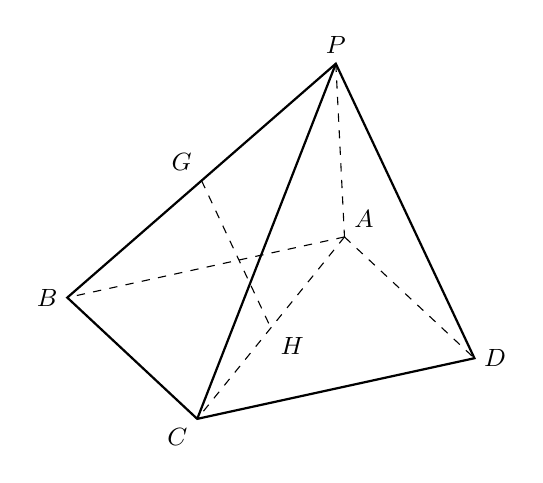
\begin{tikzpicture}[>=latex, font=\small, scale=1.1]
  % 顶点坐标
  \coordinate (P) at (1.1, 2.3);
  \coordinate (A) at (1.2, 0.3);
  \coordinate (B) at (-2.0, -0.4);
  \coordinate (C) at (-0.5, -1.8);
  \coordinate (D) at (2.7, -1.1);

  % 中点坐标
  \coordinate (G) at (-0.45, 0.95);
  \coordinate (H) at (0.35, -0.75);

  % 虚线不可见边与内部线段
  \draw[dashed, thin] (P) -- (A);
  \draw[dashed, thin] (A) -- (B);
  \draw[dashed, thin] (A) -- (D);
  \draw[dashed, thin] (A) -- (C);
  \draw[dashed, thin] (G) -- (H);

  % 实线可见外轮廓与面边界
  \draw[thick] (P) -- (B) -- (C) -- (D) -- cycle;
  \draw[thick] (P) -- (C);

  % 顶点标记
  \node[above] at (P) {$P$};
  \node[above right] at (A) {$A$};
  \node[left] at (B) {$B$};
  \node[below left] at (C) {$C$};
  \node[right] at (D) {$D$};
  \node[above left] at (G) {$G$};
  \node[below right] at (H) {$H$};
\end{tikzpicture}
\end{center}
\nopagebreak[4]
(1) 设 $G, H$ 分别为 $PB, AC$ 的中点, 求证: $GH \parallel \text{\text{平面} } PAD$;
(2) 求证: $PA \perp \text{\text{平面} } PCD$;
(3) 求直线 $AD$ 与平面 $PAC$ 所成角的正弦值.

\Needspace{4\baselineskip}
\textbf{解析}

\textbf{(1) 证明}

连接 $BD$ 交 $AC$ 于点 $H_0$。
在平行四边形 $ABCD$ 中，对角线互相平分，所以 $H_0$ 为线段 $AC$ 的中点。
已知 $H$ 为 $AC$ 的中点，因此点 $H$ 与 $H_0$ 重合，即点 $H$ 也是线段 $BD$ 的中点。
在 $\triangle PBD$ 中，$G$ 为 $PB$ 的中点，$H$ 为 $BD$ 的中点，
所以 $GH$ 为 $\triangle PBD$ 的中位线，从而 $GH \parallel PD$。
因为 $PD \subset \text{\text{平面} } PAD$，且 $GH \not\subset \text{\text{平面} } PAD$，
所以 $GH \parallel \text{\text{平面} } PAD$。

\textbf{(2) 证明}

因为平面 $PAC \perp \text{\text{平面} } PCD$，且平面 $PAC \cap \text{\text{平面} } PCD = PC$。
在平面 $PCD$ 内，过点 $C$ 作直线 $l \perp PC$。
由平面与平面垂直的性质定理，在一个平面内垂直于两平面交线的直线必垂直于另一个平面，
所以 $l \perp \text{\text{平面} } PAC$。
因为 $PA \subset \text{\text{平面} } PAC$，所以 $PA \perp l$。
又已知 $PA \perp CD$。
在等边三角形 $\triangle PCD$ 中，$\angle PCD = 60^\circ$，
而直线 $l \perp PC$，所以直线 $l$ 与直线 $CD$ 不平行，交于点 $C$。
又 $l \subset \text{\text{平面} } PCD$，$CD \subset \text{\text{平面} } PCD$。
因此 $PA$ 垂直于平面 $PCD$ 内的两条相交直线 $l$ 和 $CD$。
故 $PA \perp \text{\text{平面} } PCD$。

\textbf{(3) 解}

由 (2) 知 $PA \perp \text{\text{平面} } PCD$。
因为 $PA \subset \text{\text{平面} } PAC$，所以平面 $PAC \perp \text{\text{平面} } PCD$。
两平面的交线为 $PC$。
在等边三角形 $\triangle PCD$ 中，过点 $D$ 作 $DE \perp PC$ 于点 $E$。
因为平面 $PAC \perp \text{\text{平面} } PCD$，$DE \subset \text{\text{平面} } PCD$，且 $DE \perp PC$，
由面面垂直的性质定理可知，$DE \perp \text{\text{平面} } PAC$。
因此线段 $DE$ 的长度即为点 $D$ 到平面 $PAC$ 的距离。
已知 $\triangle PCD$ 为等边三角形，边长 $CD = 2$，
\Needspace{5\baselineskip}
所以
\nopagebreak[4]
\[DE = CD \sin 60^\circ = 2 \times \frac{\sqrt{3}}{2} = \sqrt{3}.\]
连接 $AE$。因为 $DE \perp \text{\text{平面} } PAC$，所以 $\angle DAE$ 即为直线 $AD$ 与平面 $PAC$ 所成的角。
在直角三角形 $\triangle ADE$ 中，已知 $AD = 3$，$DE = \sqrt{3}$，
\Needspace{5\baselineskip}
因此直线 $AD$ 与平面 $PAC$ 所成角的正弦值为：
\nopagebreak[4]
\[\sin\angle DAE = \frac{DE}{AD} = \frac{\sqrt{3}}{3}.\]

\gkanswer{答案（1）：证明见解析版}

\gkanswer{答案（2）：证明见解析版}

\gkanswer{答案（3）：$\dfrac{\sqrt{3}}{3}$}

\end{answer}
\begin{answer}
\gksolhead{18}{}

\textbf{题目}（本小题满分 14 分）：

设 $\{a_n\}$ 是等差数列, $\{b_n\}$ 是等比数列, 公比大于 0, 已知 $a_1 = b_1 = 3$, $b_2 = a_3$, $b_3 = 4a_2 + 3$.
(1) 求 $\{a_n\}$ 和 $\{b_n\}$ 的通项公式;
(2) 设数列 $\{c_n\}$ 满足 $c_n = \begin{cases} 1, & n \text{ \text{为奇数}}, \\ b_{\frac{n}{2}}, & n \text{ \text{为偶数}}, \end{cases}$ 求 $a_1 c_1 + a_2 c_2 + \cdots + a_{2n} c_{2n}$ ($n \in \mathbb{N}^*$).

\Needspace{4\baselineskip}
\textbf{解析}

\textbf{(1) 解}

设等差数列 $\{a_n\}$ 的公差为 $d$，等比数列 $\{b_n\}$ 的公比为 $q$ ($q > 0$)。
\Needspace{5\baselineskip}
已知 $a_1 = b_1 = 3$，则
\nopagebreak[4]
\[a_2 = 3 + d,\quad a_3 = 3 + 2d,\]
\nopagebreak[4]
\[b_2 = 3q,\quad b_3 = 3q^2.\]
\Needspace{5\baselineskip}
由已知条件 $b_2 = a_3$ 和 $b_3 = 4a_2 + 3$ 可得：
\nopagebreak[4]
\[
\begin{cases}
3q = 3 + 2d, \\
3q^2 = 4(3 + d) + 3 = 15 + 4d.
\end{cases}
\]
\Needspace{5\baselineskip}
由第一式得 $2d = 3q - 3$。代入第二式：
\nopagebreak[4]
\[3q^2 = 15 + 2(3q - 3) = 15 + 6q - 6 = 6q + 9.\]
\Needspace{5\baselineskip}
两边除以 $3$：
\nopagebreak[4]
\[q^2 - 2q - 3 = 0 \iff (q - 3)(q + 1) = 0.\]
因为公比 $q > 0$，所以 $q = 3$。
代入得公差 $d = \dfrac{3 \times 3 - 3}{2} = 3$。
\Needspace{5\baselineskip}
因此：
\nopagebreak[4]
\[a_n = a_1 + (n - 1)d = 3 + 3(n - 1) = 3n,\]
\nopagebreak[4]
\[b_n = b_1 q^{n-1} = 3 \cdot 3^{n-1} = 3^n.\]

\textbf{(2) 解}

依题意，数列 $\{c_n\}$ 的奇数项为 $1$，偶数项为 $c_{2k} = b_k = 3^k$。
\Needspace{5\baselineskip}
将和式 $S = a_1 c_1 + a_2 c_2 + \cdots + a_{2n} c_{2n}$ 拆分为奇数项之和与偶数项之和两部分：
\nopagebreak[4]
\[S = \sum_{k=1}^n a_{2k-1} c_{2k-1} + \sum_{k=1}^n a_{2k} c_{2k}.\]
\Needspace{5\baselineskip}
计算奇数项部分：
\nopagebreak[4]
\[\sum_{k=1}^n a_{2k-1} c_{2k-1} = \sum_{k=1}^n a_{2k-1} = \sum_{k=1}^n 3(2k - 1) = \sum_{k=1}^n (6k - 3) = 6 \cdot \frac{n(n + 1)}{2} - 3n = 3n^2.\]
计算偶数项部分：
各偶数项为 $a_{2k} c_{2k} = 3(2k) \cdot 3^k = 6k \cdot 3^k$。
设 $T_n = \sum_{k=1}^n 6k \cdot 3^k = 6 \sum_{k=1}^n k \cdot 3^k$。
令 $U_n = \sum_{k=1}^n k \cdot 3^k = 1 \cdot 3^1 + 2 \cdot 3^2 + \cdots + n \cdot 3^n$。
\Needspace{5\baselineskip}
采用错位相减法：
\nopagebreak[4]
\[3 U_n = 1 \cdot 3^2 + 2 \cdot 3^3 + \cdots + n \cdot 3^{n+1}.\]
\Needspace{5\baselineskip}
两式相减：
\nopagebreak[4]
\[\begin{aligned}
-2 U_n &= 3^1 + 3^2 + \cdots + 3^n - n \cdot 3^{n+1} \\
&= \frac{3(3^n - 1)}{3 - 1} - n \cdot 3^{n+1} = \frac{(1 - 2n)3^{n+1} - 3}{2}.
\end{aligned}\]
\Needspace{5\baselineskip}
两边除以 $-2$：
\nopagebreak[4]
\[U_n = \frac{(2n - 1)3^{n+1} + 3}{4}.\]
\Needspace{5\baselineskip}
从而偶数项之和为：
\nopagebreak[4]
\[T_n = 6 U_n = \frac{3[(2n - 1)3^{n+1} + 3]}{2} = \frac{(2n - 1)3^{n+2} + 9}{2}.\]
\Needspace{5\baselineskip}
将奇数项与偶数项相加，得到：
\nopagebreak[4]
\[S = 3n^2 + \frac{(2n - 1)3^{n+2} + 9}{2}.\]

\gkanswer{答案（1）：$a_n = 3n$，$b_n = 3^n$}

\gkanswer{答案（2）：$3n^2 + \dfrac{(2n - 1)3^{n+2} + 9}{2}$}

\end{answer}
\begin{answer}
\gksolhead{19}{}

\textbf{题目}（本小题满分 14 分）：

设椭圆 $\dfrac{x^2}{a^2} + \dfrac{y^2}{b^2} = 1$ ($a > b > 0$) 的左焦点为 $F$, 左顶点为 $A$, 上顶点为 $B$. 已知 $\sqrt{3}|OA| = 2|OB|$ ($O$ 为原点).
(1) 求椭圆的离心率;
(2) 设经过点 $F$ 且斜率为 $\dfrac{3}{4}$ 的直线 $l$ 与椭圆在 $x$ 轴上方的交点为 $P$, 圆 $C$ 同时与 $x$ 轴和直线 $l$ 相切, 圆心 $C$ 在直线 $x = 4$ 上, 且 $OC \parallel AP$, 求椭圆的方程.

\Needspace{4\baselineskip}
\textbf{解析}

\textbf{(1) 解}

由题意，椭圆 $\dfrac{x^2}{a^2} + \dfrac{y^2}{b^2} = 1$ ($a > b > 0$) 的左顶点为 $A(-a, 0)$，上顶点为 $B(0, b)$。
则 $|OA| = a$，$|OB| = b$。
已知 $\sqrt{3}|OA| = 2|OB|$，即 $\sqrt{3}a = 2b$。
\Needspace{5\baselineskip}
两边平方得：
\nopagebreak[4]
\[3a^2 = 4b^2 = 4(a^2 - c^2) \iff 3a^2 = 4a^2 - 4c^2 \iff 4c^2 = a^2.\]
\Needspace{5\baselineskip}
因此离心率为：
\nopagebreak[4]
\[e = \frac{c}{a} = \frac{1}{2}.\]

\textbf{(2) 解}

由 (1) 知 $c = \dfrac{1}{2}a$，$b^2 = \dfrac{3}{4}a^2$。
左顶点为 $A(-a, 0)$，左焦点为 $F\left(-\dfrac{1}{2}a, 0\right)$。
\Needspace{5\baselineskip}
直线 $l$ 经过点 $F$ 且斜率为 $\dfrac{3}{4}$，其方程为：
\nopagebreak[4]
\[y = \frac{3}{4}\left(x + \frac{a}{2}\right) \iff 3x - 4y + \frac{3a}{2} = 0.\]
\Needspace{5\baselineskip}
将直线方程代入椭圆方程 $\dfrac{x^2}{a^2} + \dfrac{y^2}{\frac{3}{4}a^2} = 1 \iff 3x^2 + 4y^2 = 3a^2$：
\nopagebreak[4]
\[3x^2 + 4 \cdot \frac{9}{16}\left(x + \frac{a}{2}\right)^2 = 3a^2 \iff 3x^2 + \frac{9}{4}\left(x^2 + ax + \frac{a^2}{4}\right) = 3a^2.\]
\Needspace{5\baselineskip}
两边同乘以 $4$ 并整理：
\nopagebreak[4]
\[12x^2 + 9x^2 + 9ax + \frac{9}{4}a^2 = 12a^2 \iff 21x^2 + 9ax - \frac{39}{4}a^2 = 0.\]
\Needspace{5\baselineskip}
两边同除以 $3$ 再乘以 $4$：
\nopagebreak[4]
\[28x^2 + 12ax - 13a^2 = 0 \iff (2x - a)(14x + 13a) = 0.\]
因为点 $P$ 在 $x$ 轴上方，$y > 0$，代入两根检验：
\begin{itemize}
\item 若 $x = -\dfrac{13}{14}a$，则 $y = \dfrac{3}{4}\left(-\dfrac{13}{14}a + \dfrac{7}{14}a\right) = -\dfrac{9}{28}a < 0$，舍去；
\item 若 $x = \dfrac{a}{2}$，则 $y = \dfrac{3}{4}\left(\dfrac{a}{2} + \dfrac{a}{2}\right) = \dfrac{3}{4}a > 0$。
\end{itemize}
因此点 $P$ 的坐标为 $P\left(\dfrac{a}{2}, \dfrac{3}{4}a\right)$。
\Needspace{5\baselineskip}
计算直线 $AP$ 的斜率：
\nopagebreak[4]
\[k_{AP} = \frac{\frac{3}{4}a - 0}{\frac{a}{2} - (-a)} = \frac{\frac{3}{4}a}{\frac{3}{2}a} = \frac{1}{2}.\]
圆心 $C$ 在直线 $x = 4$ 上，可设 $C(4, y_0)$。
\Needspace{5\baselineskip}
因为 $OC \parallel AP$，所以直线 $OC$ 的斜率等于 $k_{AP}$：
\nopagebreak[4]
\[\frac{y_0}{4} = \frac{1}{2} \implies y_0 = 2.\]
所以圆心坐标为 $C(4, 2)$。
因为圆 $C$ 与 $x$ 轴相切，所以圆的半径等于圆心纵坐标的绝对值，即 $R = 2$。
又因为圆 $C$ 与直线 $l: 3x - 4y + \dfrac{3a}{2} = 0$ 相切，
\Needspace{5\baselineskip}
圆心 $C(4, 2)$ 到直线 $l$ 的距离等于半径 $R = 2$：
\nopagebreak[4]
\[d = \frac{\left|3 \times 4 - 4 \times 2 + \frac{3a}{2}\right|}{\sqrt{3^2 + (-4)^2}} = \frac{\left|4 + \frac{3a}{2}\right|}{5} = 2.\]
即 $\left|4 + \dfrac{3a}{2}\right| = 10$。
因为 $a > 0$，所以 $4 + \dfrac{3a}{2} = 10 \implies \dfrac{3a}{2} = 6 \implies a = 4$。
从而 $a^2 = 16$，$b^2 = \dfrac{3}{4}a^2 = 12$。
\Needspace{5\baselineskip}
因此，椭圆的标准方程为：
\nopagebreak[4]
\[\frac{x^2}{16} + \frac{y^2}{12} = 1.\]

\gkanswer{答案（1）：$\dfrac{1}{2}$}

\gkanswer{答案（2）：$\dfrac{x^2}{16} + \dfrac{y^2}{12} = 1$}

\end{answer}
\begin{answer}
\gksolhead{20}{}

\textbf{题目}（本小题满分 14 分）：

设函数 $f(x) = \ln x - a(x - 1)\mathrm{e}^x$, 其中 $a \in \mathbb{R}$.
(1) 若 $a \leqslant 0$, 讨论 $f(x)$ 的单调性;
(2) 若 $0 < a < \dfrac{1}{\mathrm{e}}$,
① 证明 $f(x)$ 恰有两个零点;
② 设 $x_0$ 为 $f(x)$ 的极值点, $x_1$ 为 $f(x)$ 的零点, 且 $x_1 > x_0$, 证明 $3x_0 - x_1 > 2$.

\Needspace{4\baselineskip}
\textbf{解析}

\textbf{(1) 解}

函数 $f(x) = \ln x - a(x - 1)\mathrm{e}^x$ 的定义域为 $(0, +\infty)$。
\Needspace{5\baselineskip}
对其求导：
\nopagebreak[4]
\[f'(x) = \frac{1}{x} - a\left[\mathrm{e}^x + (x - 1)\mathrm{e}^x\right] = \frac{1}{x} - ax\mathrm{e}^x.\]
当 $a \leqslant 0$ 时，对任意 $x \in (0, +\infty)$，均有 $\dfrac{1}{x} > 0$ 且 $-ax\mathrm{e}^x \geqslant 0$。
因此 $f'(x) > 0$ 在 $(0, +\infty)$ 上恒成立。
所以当 $a \leqslant 0$ 时，$f(x)$ 在 $(0, +\infty)$ 上单调递增。

\textbf{(2) 证明}

① 考察导函数 $f'(x) = \dfrac{1}{x} - ax\mathrm{e}^x$。
\Needspace{5\baselineskip}
改写为
\nopagebreak[4]
\[f'(x) = x\mathrm{e}^x\left(\frac{1}{x^2\mathrm{e}^x} - a\right).\]
令函数 $g(x) = x^2\mathrm{e}^x$ ($x > 0$)。
因为 $g'(x) = (2x + x^2)\mathrm{e}^x > 0$，所以 $g(x)$ 在 $(0, +\infty)$ 上严格单调递增。
从而函数 $\dfrac{1}{x^2\mathrm{e}^x}$ 在 $(0, +\infty)$ 上严格单调递减，其值域为 $(0, +\infty)$。
\Needspace{5\baselineskip}
已知 $0 < a < \dfrac{1}{\mathrm{e}}$，由零点存在定理可知，存在唯一的 $x_0 \in (0, +\infty)$，使得
\nopagebreak[4]
\[\frac{1}{x_0^2\mathrm{e}^{x_0}} - a = 0 \iff f'(x_0) = 0.\]
\begin{itemize}
\item 当 $x \in (0, x_0)$ 时，$f'(x) > 0$，$f(x)$ 单调递增；
\item 当 $x \in (x_0, +\infty)$ 时，$f'(x) < 0$，$f(x)$ 单调递减。
\end{itemize}
因此 $f(x)$ 在 $x = x_0$ 处取得极大值，也是定义域内的最大值。
注意到 $f(1) = \ln 1 - a(1 - 1)\mathrm{e}^1 = 0$，即 $x = 1$ 是 $f(x)$ 的一个零点。
\Needspace{5\baselineskip}
计算 $x = 1$ 处的导数值：
\nopagebreak[4]
\[f'(1) = 1 - a\mathrm{e}.\]
因为 $0 < a < \dfrac{1}{\mathrm{e}}$，所以 $f'(1) = 1 - a\mathrm{e} > 0$。
结合 $f'(x)$ 在 $(0, +\infty)$ 上的单调性以及 $f'(x_0) = 0$，可得 $x_0 > 1$。
因此最大值满足 $f(x_0) > f(1) = 0$。
\begin{itemize}
\item 在区间 $(0, x_0)$ 上，$f(x)$ 单调递增，且 $f(1) = 0$，故在该区间内有且仅有唯一零点 $x = 1$；
\item 在区间 $(x_0, +\infty)$ 上，$f(x)$ 单调递减，且 $f(x_0) > 0$。
\end{itemize}
  当 $x \to +\infty$ 时，$\lim_{x \to +\infty} \left[\ln x - a(x - 1)\mathrm{e}^x\right] = -\infty$。
  由零点存在定理，在 $(x_0, +\infty)$ 内存在唯一的零点。
综合可知，当 $0 < a < \dfrac{1}{\mathrm{e}}$ 时，$f(x)$ 恰有两个零点。

② 设 $x_1$ 为 $f(x)$ 在 $(x_0, +\infty)$ 内的零点，即 $x_1 > x_0$ 且 $f(x_1) = 0$。
\Needspace{5\baselineskip}
因为 $x_0$ 是极值点，满足 $f'(x_0) = 0$，即
\nopagebreak[4]
\[a = \frac{1}{x_0^2\mathrm{e}^{x_0}}.\]
\Needspace{5\baselineskip}
代入 $f(x)$ 的解析式：
\nopagebreak[4]
\[f(x) = \ln x - \frac{x - 1}{x_0^2}\mathrm{e}^{x - x_0}.\]
因为 $f(x)$ 在 $(x_0, +\infty)$ 上单调递减，且 $f(x_1) = 0$，
要证明 $3x_0 - x_1 > 2 \iff x_1 < 3x_0 - 2$，
注意到 $x_0 > 1 \implies 3x_0 - 2 > x_0$，即 $3x_0 - 2 \in (x_0, +\infty)$。
\Needspace{5\baselineskip}
由单调性，只需证明
\nopagebreak[4]
\[f(3x_0 - 2) < f(x_1) = 0.\]
\Needspace{5\baselineskip}
将 $x = 3x_0 - 2$ 代入 $f(x)$：
\nopagebreak[4]
\[f(3x_0 - 2) = \ln(3x_0 - 2) - \frac{3x_0 - 3}{x_0^2}\mathrm{e}^{2(x_0 - 1)} = \ln(1 + 3(x_0 - 1)) - \frac{3(x_0 - 1)}{x_0^2}\mathrm{e}^{2(x_0 - 1)}.\]
令 $t = x_0 - 1$。因为 $x_0 > 1$，所以 $t > 0$，$x_0 = 1 + t$。
\Needspace{5\baselineskip}
上式化为关于 $t > 0$ 的函数：
\nopagebreak[4]
\[\varphi(t) = \ln(1 + 3t) - \frac{3t}{(1 + t)^2}\mathrm{e}^{2t}.\]
\Needspace{5\baselineskip}
由常见不等式 $\ln(1 + u) < u$ ($u > 0$)，取 $u = 3t$ 得：
\nopagebreak[4]
\[\ln(1 + 3t) < 3t.\]
\Needspace{5\baselineskip}
又对任意 $t > 0$，利用 Taylor 展开放缩：
\nopagebreak[4]
\[\mathrm{e}^{2t} > 1 + 2t + \frac{(2t)^2}{2} = 1 + 2t + 2t^2 > 1 + 2t + t^2 = (1 + t)^2.\]
\Needspace{5\baselineskip}
两边除以 $(1 + t)^2$ 得：
\nopagebreak[4]
\[\frac{\mathrm{e}^{2t}}{(1 + t)^2} > 1.\]
\Needspace{5\baselineskip}
因为 $3t > 0$，所以
\nopagebreak[4]
\[\frac{3t}{(1 + t)^2}\mathrm{e}^{2t} > 3t.\]
\Needspace{5\baselineskip}
综合上述放缩，对任意 $t > 0$，均有：
\nopagebreak[4]
\[\varphi(t) = \ln(1 + 3t) - \frac{3t}{(1 + t)^2}\mathrm{e}^{2t} < 3t - 3t = 0.\]
因此 $f(3x_0 - 2) < 0$ 恒成立。
结合 $f(x)$ 在 $(x_0, +\infty)$ 上的单调递减性，即得 $x_1 < 3x_0 - 2$。
故 $3x_0 - x_1 > 2$ 得证。

\gkanswer{答案（1）：$f(x)$ 在 $(0, +\infty)$ 上单调递增}

\gkanswer{答案（2）：① 证明见解析版；② 证明见解析版}

\end{answer}